%!TEX root = practicum2.tex
This section presents our exploration of the parameter space of the percolation model. In \cref{ss:exp:probability} we discuss the influence of the probability parameter $p$. In this section we often use the size of the cluster to compare the influence of the different parameters. We have defined the cluster size as the number of points that is occupied. 

\Cref{ss:exp:systemSize} explores the effect of the size of the system on the generated clusters. In \cref{ss:exp:fractal} we attempt to determine the fractal dimension of the finite clusters as a function of $p$. Finally, \cref{ss:exp:connectivity} presents a short analysis of the impact of the used connectivity.


\subsection{Probability}
\label{ss:exp:probability}
%!TEX root = practicum2.tex
\begin{figure}%[b!]
	\centering
	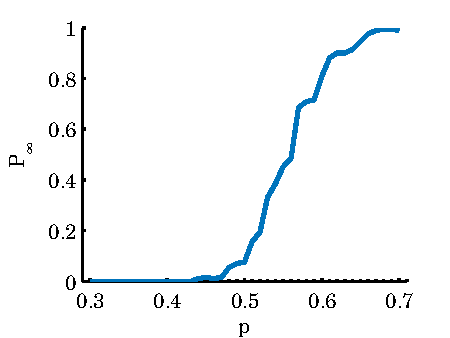
\includegraphics[width=\columnwidth]{./img/assignment_a_p_infinite_ratio_p.pdf}
	\caption{Ratio of percolating clusters, $P_\infty$, as a function of $p$. Ratios are calculated over $r_{max} = 200$ runs on a $41 \times 41$ grid.}
	\label{fig:experiment:prob:p_inf_ratio}
\end{figure}


% \begin{figure*}
% 	\centering
% 	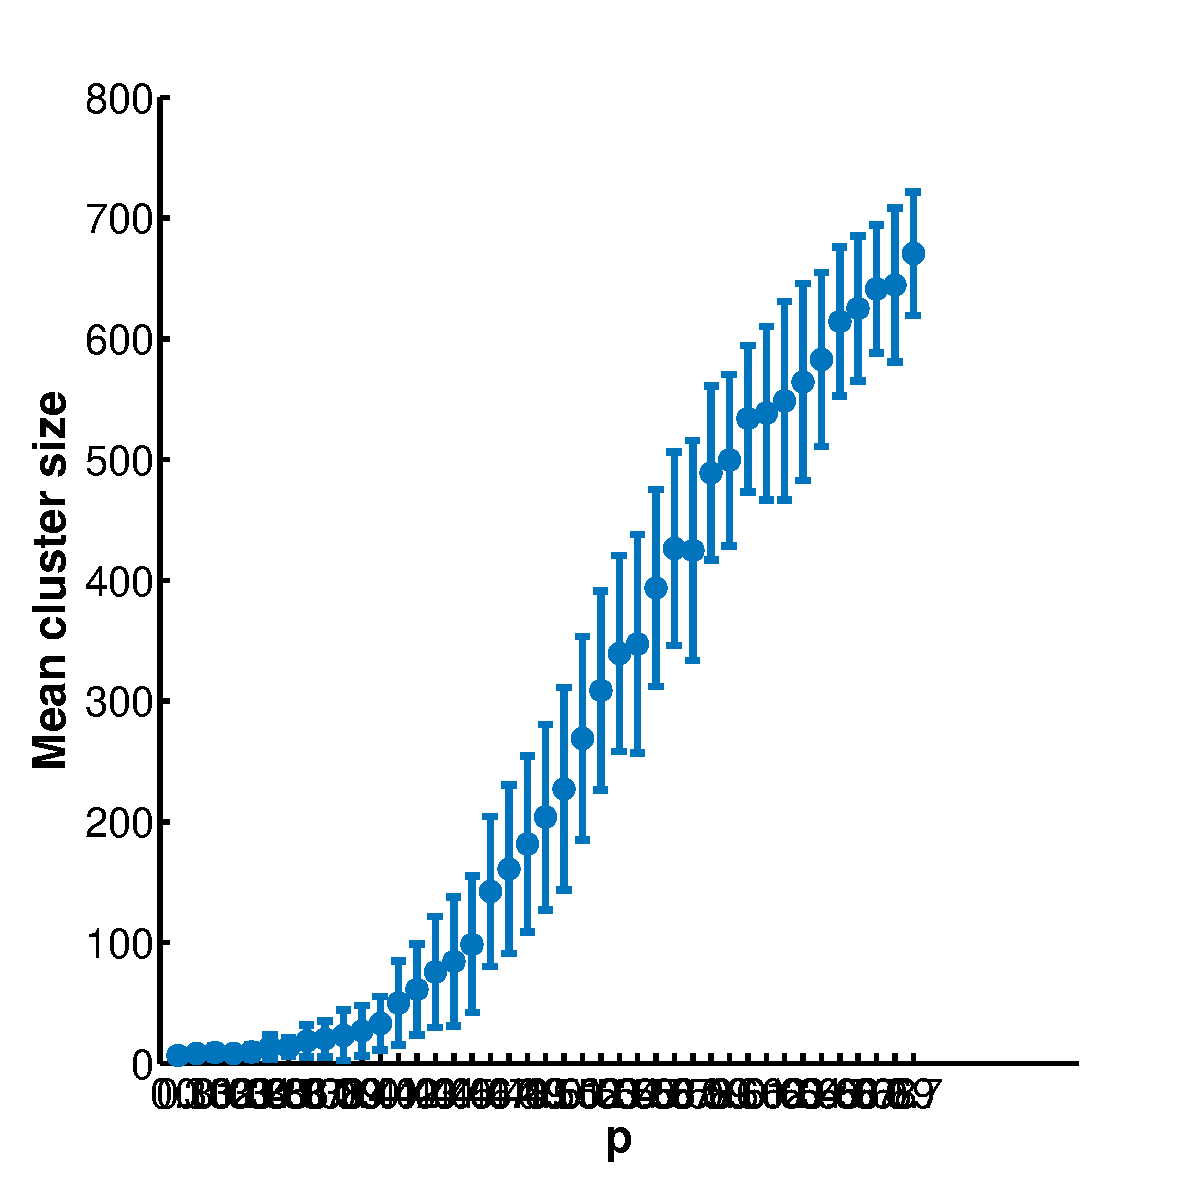
\includegraphics[width=\textwidth]{./img/assignment_a_mean_std_p.pdf}
% 	\caption{Mean cluster sizes, represented as points, and standard deviations, indicated by the vertical error bars, as a function of $p$, with a step size of $0.1$. The mean and standard deviation were calculated over $200$ runs on a $41 \times 41$ grid.}
% 	\label{fig:experiment:prob:mean_std_clusters}
% \end{figure*}

% Theory
One important property of clusters is their size, and how that size depends on the parameter $p$. As noted before the size of percolating cluster is not meaningfull, therefore do not consider percolating clusters in the following discussion. \textcite{kenzel1997physics} describe the relation between the size of a cluster and the paramter $p$ as follows: for small values of $p$ we get a large number of small clusters. As $p$ increases we find positive correlation between $p$ and the average cluster size until $p$ reaches some threshold value $p_c$. For $p > p_c$ we get either a small finite cluster or a percolating cluster. As $p > p_c$ increases the probability of finding a finite cluster decreases, until we always get a percolating cluster for $p =1 $. Note that although in theory this cluster should cover the full grid, this is not necessarily the case in our model, since it stops growing as soon as one border site is occupied.\\

% Ons experiment
To find an indication of the value of $p_c$ with our model we have let it generate a cluster on a $41 \times 41$ grid for $p = 0.30, 0.31, \dotsc, 0.7$. For each value of $p$ we grow $r_{max} = 200$ clusters. 

\Cref{fig:experiment:prob:mean_std_clusters} presents the mean and standard deviation of the size of the finite clusters as a function of $p$. In this figure we observe the effect of $p$ on the mean cluster size described by \citeauthor{kenzel1997physics}. Furthermore, based on these data one would estimate $p_c$ to be approximately $0.55$. 

\citeauthor{kenzel1997physics} also predicted that the number of percolating clusters relative to the number of finite clusters would grow for $p > p_c$ until $p = 1$, where the only possibility would be a percolating cluster. To observe this effect \cref{fig:experiment:prob:p_inf_ratio} shows $P_\infty$, which is the ratio of the number of percolating clusters to the number of finite clusters. This graph is based on the same data as \cref{fig:experiment:prob:mean_std_clusters}. Based on this graph we would say that $p_c \approx 0.4$. This number is lower than the value for $p_c$ based on \cref{fig:experiment:prob:mean_std_clusters}. This is probably caused by the relatively small grid sizes, which causes us to classify some clusters as percolating, that are actually finite. 

\textcite{stauffer1994introduction} has found $p_c$ to be approximately \num{0.59275} for a square lattice. As stated earlier our lower estimation of $p_c$ is quite likely caused by our small grid. 


\subsection{System Size}
\label{ss:exp:systemSize}
%!TEX root = practicum2.tex
% \begin{figure*}
% 	\centering
% 	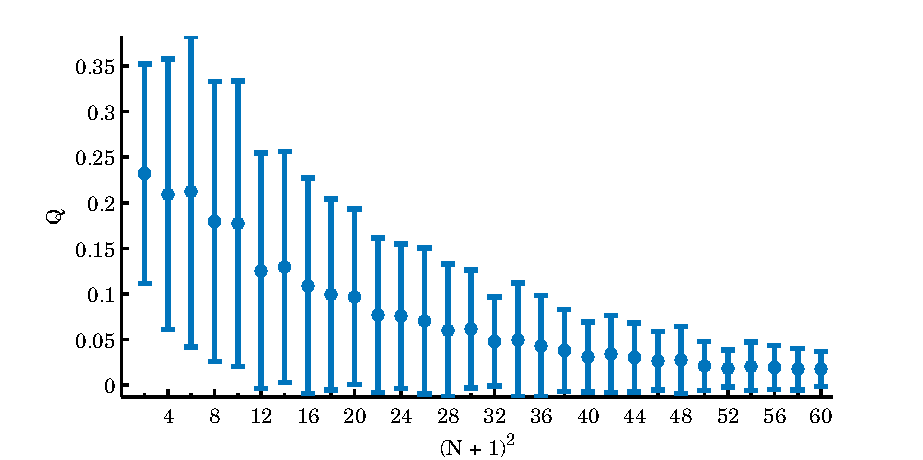
\includegraphics[width=\textwidth]{./img/assignment_b_mean_std_n.pdf}
% 	\caption{The mean, represented as points, and standard deviations, indicated by the error bars, of the ratio of the cluster size to number of sites in the grid, i.e. $(N + 1)^2$.The mean and standard deviation were calculated over $200$ runs with $p = 0.5$.}
% 	\label{fig:experiment:size:mean_std_clusters}
% \end{figure*}

In \cref{ss:exp:probability} we postulated that our relatively small grid influenced the found value of $p_c$. This section qualitatively discusses the relation between the size of the grid and the cluster. We repeat the experiment discussed in \cref{ss:exp:probability} but varied $N = 2, 6, \dotsc, 60$ instead of $p$. Since we are mostly interested in the size of finite clusters we choose $p = 0.5 < p_c$. Instead of the size of grid we now measure $Q$ the ratio of the size of finite clusters to the number of sites in the grid. 

\Cref{fig:experiment:size:mean_std_clusters} in \cref{ap:ss:size} shows the mean and standard deviation of $Q$ as a function of $N$. In this graph we observe that the average of $Q$ decreases as $N$ increases, i.e. the size of the clusters does not grow as hard as the number of sites in the grid. \todo{Physics by computer heeft een hoop theorie hiervoer die ik niet helemaal begrijp... of waarvoor we in ieder geval een ander soort plotjes moeten maken.} 

\Cref{fig:experiment:size:prob:p_inf_ratio} shows that $P_\infty$ reaches zero for $N > 40$, which indicates that for this value of $N$ there are no more percolating clusters. This fits with the theory discussed in \cref{ss:exp:probability}, which states that we get only finite clusters for $p < p_c$. We have percolating clusters for $p = 0.5 < p_c$ since the grid is not large enough to hold the finite clusters.\\ 

\begin{figure}
	\centering
	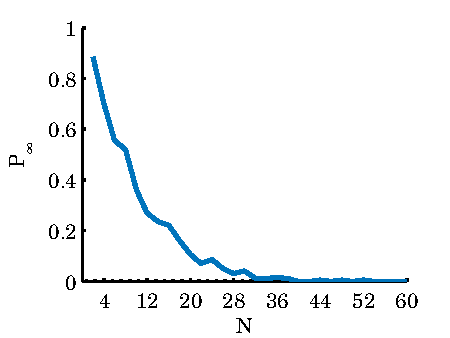
\includegraphics[width=\columnwidth]{./img/assignment_b_p_infinite_ratio_p.pdf}
	\caption{Ratio of percolating clusters to the number of finite clusters, $P_\infty$, as a function of $N$. Ratios are calculated over $r_{max} = 200$ runs with $p = 0.5$.}
	\label{fig:experiment:size:prob:p_inf_ratio}
\end{figure}

% Behaviour in the limit. 
If the lattice size is infinite we are no longer limited by the size of the lattice, in essence we remove one of our stop conditions. In this situation the theory presented in \cref{ss:exp:probability} holds, i.e. as long as $p < p_c$ we only have finite clusters. As $p > p_c$ the number of percolating clusters relative to the number of finite clusters increases until we always get a percolating cluster for $p = 1$.

	

\subsection{Fractal Dimension}
\label{ss:exp:fractal}
%!TEX root = practicum2.tex
\todo[inline]{Hoe verandert de fractal dimension $\rho$ als een functie van $p$? Ik het geprobeerd, zie branch fractalDimension, maar ik krijg dimensions eruit die allemaal lager zijn dan wat het hoort te zijn en het plotten gaat volledig stuk. In boxcount staat onderaan een functie de de fractal dimension berekent, op het moment gebruikt die de mean van de gradient, maar volgens Biehl zou je lineare regressie moeten gebruiken. Allebei geven ze crap resulaten.}

\begin{figure*}
	\centering
	\begin{subfigure}[t]{0.3\textwidth}
		\centering
		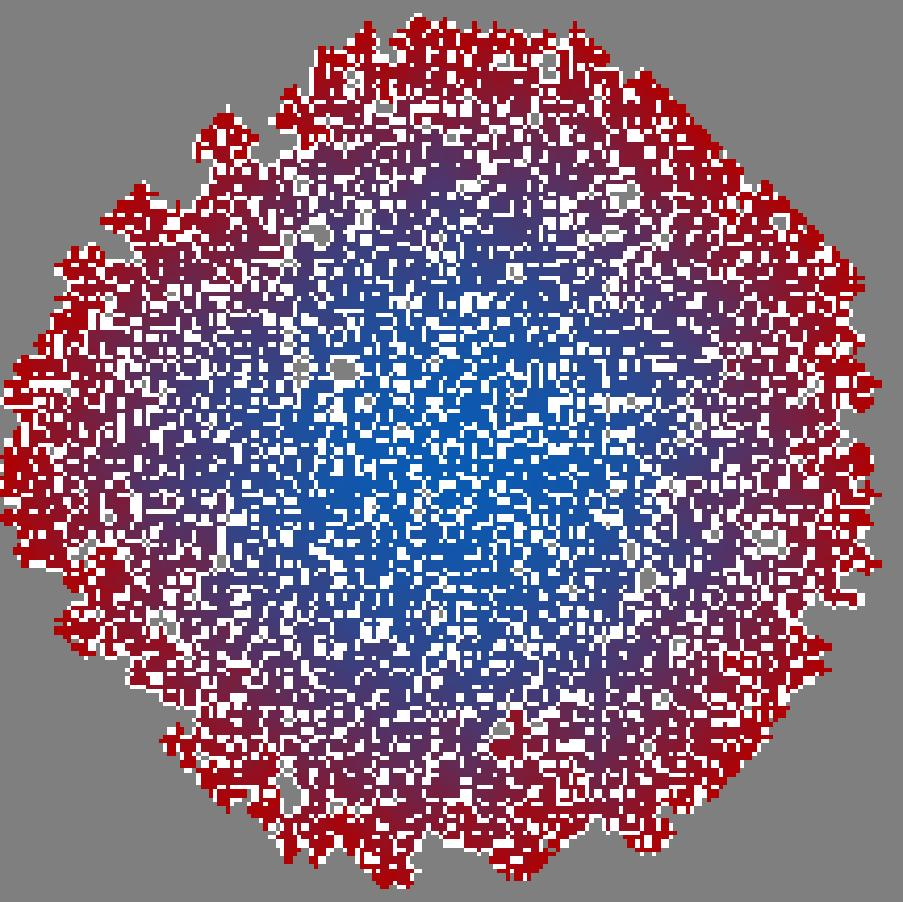
\includegraphics[width=1\textwidth]{./img/assignment_fractal_cluster}
		\caption{The cluster.}
		\label{fig:exp_fractal:cluster}
	\end{subfigure}
	\begin{subfigure}[t]{0.3\textwidth}
		\centering
		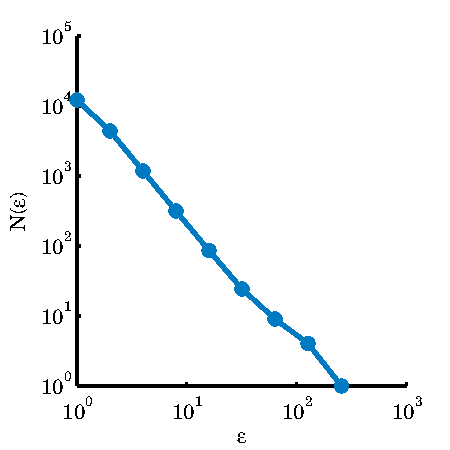
\includegraphics[width=1\textwidth]{./img/assignment_fractal_numboxesVSboxsize}
		\caption{The number of boxes as function of the box size.}
		\label{fig:exp_fractal:fractalDimension}	
	\end{subfigure}	
	\begin{subfigure}[t]{0.3\textwidth}
		\centering
		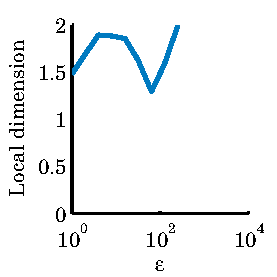
\includegraphics[width=1\textwidth]{./img/assignment_fractal_gradient}
		\caption{The minus gradient of \cref{fig:exp_fractal:fractalDimension}.}
		\label{fig:exp_fractal:fractalDimensionGradient}
	\end{subfigure}		
	\caption{\subref{fig:exp_fractal:cluster} The cluster ($N = 80, p = 0.7$) used to compute the box-counting dimension. \subref{fig:exp_fractal:fractalDimension} The number of boxes used to cover that cluster as a function of the box size. \subref{fig:exp_fractal:fractalDimensionGradient} The gradient of the function plotted in \subref{fig:exp_fractal:fractalDimension}.}
	\label{fig:exp:dimension:plaatjes}
\end{figure*}

\textcite{falconer2004fractal} describes the fractal dimension as some number $\rho$ such that
\begin{equation}
	M_\varepsilon(\rho) \sim c\varepsilon^{-s}
\end{equation}
where $c$ and $s$ are constants and $M_\varepsilon(\rho)$ are measurements at different scales $\varepsilon$ for $\varepsilon \to 0$. \citeauthor{falconer2004fractal} then shows that the fractal dimension can be estimated ``as minus the gradient of a log-log graph plotted over a suitable range of $\varepsilon$"\cite{falconer2004fractal}. 

	% \begin{equation}
	% 	\text{dim}_{\text{box}} = \lim_{\epsilon \to 0} \frac{\log N(\epsilon)}{\log\left[ \frac{1}{\epsilon} \right]}.
	% \end{equation}
One way to get the measurements $M_\varepsilon$ is to use box-counting. When one uses this algorithm the different scales mentioned in \citeauthor{falconer2004fractal}'s definition are the sizes of the boxes.

We have used the function \t{box-count} by \textcite{boxCounting} to determine the fractal dimension of one percolation cluster. This implementation of the box-counting algorithm uses box sizes that are a power of two, consequently $\varepsilon = 1, 2, 4, \dotsc 2^q$ where $q$ is the smallest integer such that $q \leq (2N + 1)$. 

\Cref{fig:exp_fractal:cluster} shows the cluster of which we have determined the fractal dimension using box-counting. It was generated with $N = 80$, $p = 0.7$. \Cref{fig:exp_fractal:fractalDimension} presents the number of boxes as a function of the size of the boxes, \cref{fig:exp_fractal:fractalDimensionGradient} presents the minus of the gradient of \cref{fig:exp_fractal:fractalDimension}. From this graph we can infer the box-counting dimension by finding the local dimension for which the gradient is approximately stable. Using this method we find the fractal dimension to be \num{1.879}, which neatly approximates the dimension \num{1.896} mentioned by \textcite{stauffer1994introduction}. The small difference between these numbers can be explained by the relatively small size of our cluster and the fact that we present the fractal dimension of only cluster instead of the average over multiple clusters. 	

\subsection{Connectivity}
\label{ss:exp:connectivity}
%!TEX root = practicum2.tex
\begin{figure}%[b!]
	\centering
	\begin{subfigure}{0.45\columnwidth}
		\centering
		
\includegraphics[width=\textwidth]{img/assignment_connectivity_four_N80_p3.jpeg}
		\caption{4-connectivity}
		\label{fig:exp:connectivity:fourConnect}
	\end{subfigure}
	\begin{subfigure}{0.45\columnwidth}
		\centering
		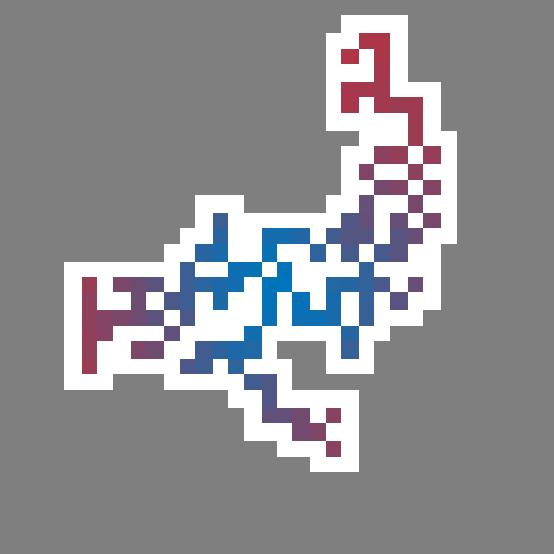
\includegraphics[width=\textwidth]{img/assignment_connectivity_eight_N80_p3.jpeg}
		\caption{8-connectivity}
		\label{fig:exp:connectivity:eightConnect}
	\end{subfigure}	
	\caption{The results of growing a cluster with the same grid of probabilites with \subref{fig:exp:connectivity:fourMask} four-connectivity and \subref{fig:exp:connectivity:eightMask} eight-connectivity. Note that although the clusters are generated on a grid with $N = 80$, we have plotted them on a grid with $N = 16$.}
	\label{fig:exp:connectivityResults}
\end{figure}

We consider two different connectivities, namely four- and eight-connectivity, which are illustrated in \cref{fig:exp:connectivity}. In this section we discuss the influence of the 8-connectivity on the size of the cluster.

\Cref{fig:exp:connectivityResults} shows two clusters which have been grown using the same probabilities but different connectivities. We see that in this case the 8-connected cluster is much larger than the 4-connected cluster. Although a different seed for the algorithms may result in different clusters in general one would expect the 8-connected cluster to grow larger than the 4-connected version. Since the expected number of sites that are occupied in each grow step when 8-connectivity is used is twice as high as the expected number of occupied sites with 4-connectivity. 

% Influence of probability
The results of performing the same experiment as discussed in \cref{ss:exp:probability} with the eight-connectivity mask, are presented in \cref{fig:experiment:conn:mean_std_clusters} in \cref{ap:ss:Connectivity} and \cref{fig:experiment:conn:p_inf_ratio}. We have changed the range of $p$ to $p = 0.2, 0.21, \dotsc, 0.6$, since even for $p = 0.3$ $P_\infty$ was close to zero. 

\begin{figure}%[b!]
	\centering
	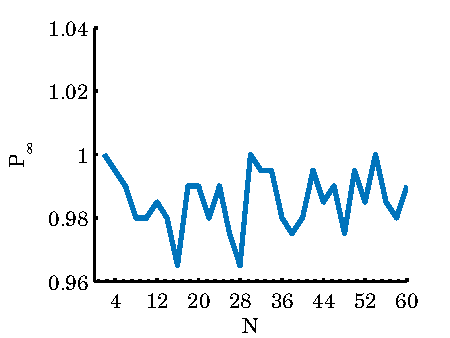
\includegraphics[width=\columnwidth]{./img/assignment_d_p_infinite_ratio_p.pdf}
	\caption{Ratio of percolating clusters, $P_\infty$, as a function of $p = 0.2, 0.21, \dotsc, 0.6$ when eight-connectivity is used. Ratios are calculated over $r_{max} = 200$ runs on a $41 \times 41$ grid.}
	\label{fig:experiment:conn:p_inf_ratio}
\end{figure}

% \begin{figure*}
% 	\centering
% 	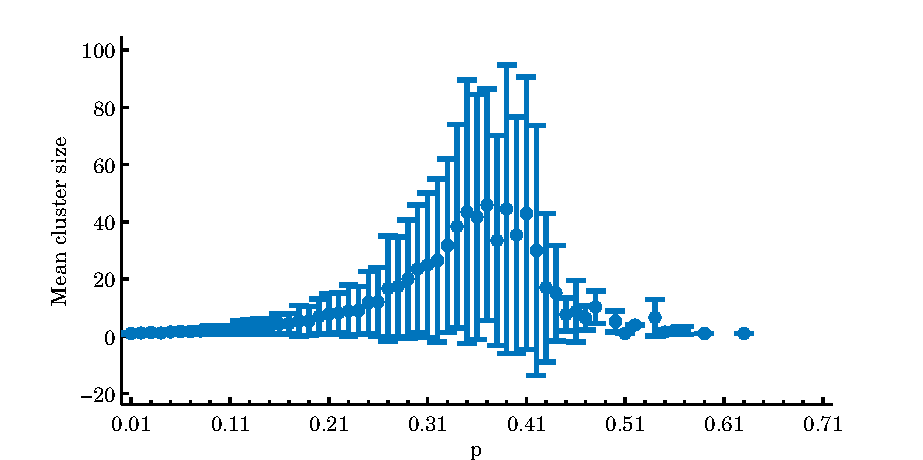
\includegraphics[width=\textwidth]{./img/assignment_d_mean_std_p.pdf}
% 	\caption{Mean cluster sizes, represented as points, and standard deviations, indicated by the vertical error bars, as a function of $p = 0.2, 0.21, \dotsc, 0.6$ when eight-connectivity is used. The mean and standard deviation were calculated over $200$ runs on a $41 \times 41$ grid.}
% 	\label{fig:experiment:conn:mean_std_clusters}
% \end{figure*}

It should be noted that for some values of $p$, especially larger values there are no mean cluster sizes, since no finite clusters were found. This indicates that one is much more likely to encounter a percolating cluster with eight-connectivity than with four-connectivity for the same value of $p$. Which fits with our ealier observation that the expected number of newly occupied sites with eight-connectivity is twice as high when compared with a four-connected cluster.

That for higher values of $p$ a percolating cluster is more likely than a finite cluster is confirmed by \cref{fig:experiment:conn:p_inf_ratio}, where we find that only for very low values of $p$ $P_\infty$ is zero, and that $P_\infty$ quickly approaches 1. 

These findings suggest that $p_c$ is much lower when eight-connectivity is used. Based on this, admittedly small experiment, one would guess $p_c$ to be approximately $0.2$ when eight-connectivity is used. More research is needed to find the actual value of $p_c$ for eight-connected clusters.\\


% \todo{Influence of size}
% % To determine the influence of the connectivity on the size we have performed the same experiment as used for the four-connectivity. \todo[inline]{Resultaten}

% \todo{Influence on fractal dimension}
% % We have determined the fractal dimension of the cluster generated using four connectivity for $N = 80$ and $p =0.7$. We have found that \todo[inline]{Resulaten}


